% =====================================================================
%  Deep Q-Learning em Haskell puro: slides do grupo em Beamer
%  Compilador no Overleaf: pdfLaTeX (Menu > Settings > Compiler)
%  Arquivos do projeto: main.tex e media-movel.dat (curva do slide de resultados)
% =====================================================================
\documentclass[aspectratio=169,10pt]{beamer}

% ---------- Idioma, codificação e fontes ----------
\usepackage[brazil]{babel}
\usepackage[utf8]{inputenc}
\usepackage[T1]{fontenc}
\usepackage[sfdefault,lf]{FiraSans}   % texto: Fira Sans
\usepackage[scaled=0.86]{FiraMono}    % código: Fira Mono
\usepackage{newtxsf}                  % matemática sem serifa, combina com a Fira
\usefonttheme{professionalfonts}

% ---------- Pacotes ----------
\usepackage{booktabs}
\usepackage{tabularx}
\usepackage{amsmath}
\usepackage[most]{tcolorbox}
\usepackage{tikz}
\usetikzlibrary{calc,positioning,shadows}
\usepackage{pgfplots}
\pgfplotsset{compat=1.18}

% ---------- Paleta ----------
\definecolor{marinho}{HTML}{1D1E3C}   % fundo dos slides escuros
\definecolor{marinho2}{HTML}{282B4C}  % cartões nos slides escuros
\definecolor{marinho3}{HTML}{3A3E68}  % bordas nos slides escuros
\definecolor{creme}{HTML}{F6F4EF}     % fundo claro
\definecolor{lavanda}{HTML}{EEECF8}   % fundo lavanda
\definecolor{linha}{HTML}{E2E0EA}     % bordas dos cartões claros
\definecolor{tinta}{HTML}{1D1E3C}     % texto principal
\definecolor{cinza}{HTML}{6B6D86}     % texto secundário
\definecolor{cinzaclaro}{HTML}{B9BBD3}% texto secundário no escuro
\definecolor{roxo}{HTML}{5B44D6}      % destaque
\definecolor{lilas}{HTML}{B8A7F2}     % destaque no escuro
\definecolor{laranja}{HTML}{E8812F}   % haste e saídas da rede

% ---------- Tema do Beamer ----------
\setbeamertemplate{navigation symbols}{}
\setbeamersize{text margin left=9mm,text margin right=9mm}
\setbeamercolor{background canvas}{bg=creme}
\setbeamercolor{normal text}{fg=tinta}
\setbeamercolor{frametitle}{fg=tinta}
\setbeamercolor{kicker}{fg=roxo}
\setbeamercolor{rodape}{fg=cinza}
\setbeamercolor{barra}{fg=roxo,bg=linha}
\setbeamercolor{itemize item}{fg=roxo}
\setbeamercolor{enumerate item}{fg=roxo}
\setbeamertemplate{itemize item}{\small\raise0.25ex\hbox{\textbullet}}
\setbeamertemplate{enumerate item}{\insertenumlabel.}

% Título do slide: rótulo pequeno (subtítulo) em cima, título grande embaixo
\makeatletter
\setbeamertemplate{frametitle}{%
  \vspace*{3mm}%
  \ifx\insertframesubtitle\@empty\else
    {\usebeamercolor[fg]{kicker}\ttfamily\tiny\bfseries\insertframesubtitle}\par\vspace{1.3mm}%
  \fi
  {\usebeamercolor[fg]{frametitle}\Large\bfseries\insertframetitle}\par
  \vspace{1mm}}
\makeatother

% Rodapé: nome do trabalho, número do slide e barra de progresso
\setbeamertemplate{footline}{%
  \ifnum\insertframenumber=1\else
  \begin{tikzpicture}[remember picture,overlay]
    \usebeamercolor{barra}
    \fill[bg] (current page.south west) rectangle ([yshift=0.7mm]current page.south east);
    \fill[fg] (current page.south west) rectangle
      ([yshift=0.7mm]$(current page.south west)!{\insertframenumber/\inserttotalframenumber}!(current page.south east)$);
    \node[anchor=south west,inner sep=0pt,font=\tiny] at ([xshift=9mm,yshift=3mm]current page.south west)
      {\usebeamercolor[fg]{rodape}Deep Q-Learning em Haskell puro};
    \node[anchor=south east,inner sep=0pt,font=\tiny\ttfamily] at ([xshift=-9mm,yshift=3mm]current page.south east)
      {\usebeamercolor[fg]{rodape}\insertframenumber\,/\,\inserttotalframenumber};
  \end{tikzpicture}%
  \fi
  \vspace*{9mm}}

% Variações de fundo. Uso: {\escuro \begin{frame}...\end{frame}}
\newcommand{\escuro}{%
  \setbeamercolor{background canvas}{bg=marinho}%
  \setbeamercolor{normal text}{fg=white}%
  \setbeamercolor{frametitle}{fg=white}%
  \setbeamercolor{kicker}{fg=lilas}%
  \setbeamercolor{rodape}{fg=cinzaclaro}%
  \setbeamercolor{barra}{fg=lilas,bg=marinho3}%
  \usebeamercolor[fg]{normal text}}
\newcommand{\lavanda}{\setbeamercolor{background canvas}{bg=lavanda}}

% ---------- Cartões (tcolorbox) ----------
% \ct{título}{texto}: título em negrito e texto menor, nas cores do cartão
\newcommand{\ct}[2]{{\footnotesize\bfseries\color{cttit}#1}\par\vspace{0.6mm}{\color{cttxt}#2}}
% \rotulo{TEXTO}: etiqueta pequena em fonte mono
\newcommand{\rotulo}[1]{{\ttfamily\tiny\bfseries\color{ctrot}#1}\par\vspace{0.8mm}}
% \modulo{texto}: nome de módulo, em mono e na cor de destaque
\newcommand{\modulo}[1]{{\ttfamily\tiny\color{ctrot}#1}}

\tcbset{
  base/.style={enhanced,arc=1.8mm,boxrule=0.5pt,left=2.4mm,right=2.4mm,top=1.5mm,bottom=1.5mm,
               fontupper=\scriptsize\raggedright,before skip=0pt,after skip=0pt},
  claro/.style={base,colback=white,colframe=linha,
               before upper={\colorlet{cttit}{tinta}\colorlet{cttxt}{cinza}\colorlet{ctrot}{roxo}}},
  clarodestaque/.style={claro,colframe=roxo,boxrule=0.9pt},
  noescuro/.style={base,colback=marinho2,colframe=marinho3,
               before upper={\colorlet{cttit}{white}\colorlet{cttxt}{cinzaclaro}\colorlet{ctrot}{lilas}}},
  noescurodestaque/.style={noescuro,colframe=lilas,boxrule=0.9pt},
  codigo/.style={base,colback=marinho,colframe=marinho,fontupper=\small\raggedright\color{white},
               left=3.5mm,right=3.5mm,top=2.5mm,bottom=2.5mm,
               before upper={\colorlet{cttit}{white}\colorlet{cttxt}{cinzaclaro}\colorlet{ctrot}{lilas}}},
  codigoescuro/.style={codigo,colback=marinho2,colframe=marinho3,boxrule=0.5pt},
}
\newtcolorbox{cartao}[1][]{claro,#1}
\newtcolorbox{cartaoD}[1][]{clarodestaque,#1}
\newtcolorbox{cartaoE}[1][]{noescuro,#1}
\newtcolorbox{cartaoED}[1][]{noescurodestaque,#1}
\newtcolorbox{codigo}[1][]{codigo,#1}
\newtcolorbox{codigoE}[1][]{codigoescuro,#1}
% Grade de cartões com a mesma altura
\newenvironment{grade}[1]{\begin{tcbraster}[raster columns=#1,raster equal height=rows,
  raster column skip=2.2mm,raster row skip=1.8mm]}{\end{tcbraster}}

% Cabeçalho de tabela
\newcommand{\cab}[1]{\leavevmode\textcolor{cinza}{\scriptsize #1}}
% Comentário pequeno e cinza dentro das caixas de fórmula
\newcommand{\nota}[1]{{\scriptsize\color{cttxt}#1}}
% Texto de rodapé do slide (conclusão)
\newcommand{\conclusao}[1]{{\footnotesize\raggedright #1\par}}

% Estilo dos gráficos
\pgfplotsset{
  estilo/.style={
    axis lines=left, axis line style={draw=cinza!60},
    tick style={draw=none}, tick label style={font=\tiny\color{cinza}},
    label style={font=\tiny\color{cinza}},
    /pgf/number format/use comma, /pgf/number format/1000 sep={.},
  }
}

% Macros de slides específicos (ficam no preâmbulo: dentro do frame o # quebra)
\newcommand{\passo}[3]{{\Large\bfseries\color{roxo}#1}\par\vspace{0.6mm}{\footnotesize\bfseries #2}\par\vspace{0.8mm}\modulo{#3}}
\newcommand{\etapa}[2]{\begin{cartao}[top=0.8mm,bottom=0.8mm]\makebox[7mm][l]{\large\bfseries\color{roxo}#1}{\footnotesize #2}\end{cartao}}
\newcommand{\numero}[1]{{\fontsize{20}{22}\selectfont\bfseries\color{lilas}#1}\par\vspace{0.8mm}}

\title{Deep Q-Learning em Haskell puro}

% =====================================================================
\begin{document}

% ---------------------------------------------------------------------
% 1. Capa
{\escuro
\begin{frame}[plain]
  \begin{tikzpicture}[remember picture,overlay]
    % rede estilizada no canto, só decoração
    \begin{scope}[shift={([xshift=-38mm,yshift=-4mm]current page.east)},opacity=0.55]
      \foreach \i in {0,...,3} \coordinate (e\i) at (0,{(\i-1.5)*0.75});
      \foreach \i in {0,...,6} \coordinate (o\i) at (1.6,{(\i-3)*0.55});
      \foreach \i in {0,1} \coordinate (s\i) at (3.2,{(\i-0.5)*0.9});
      \foreach \a in {0,...,3} \foreach \b in {0,...,6} \draw[marinho3,line width=0.3pt] (e\a)--(o\b);
      \foreach \a in {0,...,6} \foreach \b in {0,1} \draw[marinho3,line width=0.3pt] (o\a)--(s\b);
      \foreach \i in {0,...,3} \fill[roxo] (e\i) circle (1.3mm);
      \foreach \i in {0,...,6} \fill[cinzaclaro] (o\i) circle (1.1mm);
      \foreach \i in {0,1} \fill[laranja] (s\i) circle (1.3mm);
    \end{scope}
  \end{tikzpicture}
  \vspace*{6mm}
  {\ttfamily\tiny\bfseries\color{lilas}TRABALHO EM GRUPO · HASKELL}\par\vspace{3mm}
  {\fontsize{30}{33}\selectfont\bfseries Deep Q-Learning\\ em {\color{lilas}Haskell puro}}\par\vspace{4mm}
  \begin{minipage}{0.62\textwidth}
    {\small\color{cinzaclaro}Um agente aprende a equilibrar o CartPole com uma rede neural escrita do zero, só com listas.}
  \end{minipage}\par\vfill
  {\tiny\color{cinzaclaro}Raphael Resende · Bruno Santana · Felipe Massola · João Vítor Cruz · João Gabriel Ferreira · Guilherme Grati · Gabriel Fagundes · Lucas Conceição · Helena Ramos}
  \vspace*{3mm}
\end{frame}
}

% ---------------------------------------------------------------------
% 2. O problema
\begin{frame}{CartPole: equilibrar uma haste num carrinho}{O PROBLEMA}
  \begin{columns}[c,onlytextwidth]
    \begin{column}{0.44\textwidth}
      \centering
      \begin{tikzpicture}[scale=1]
        \draw[cinza,line width=0.8pt] (-2.6,0)--(2.6,0);              % trilho
        \draw[cinza!50,dashed] (0,0.75)--(0,3.1);                      % vertical de referência
        \fill[roxo,rounded corners=1.5pt] (-0.75,0.22) rectangle (0.75,0.75); % carrinho
        \fill[tinta] (-0.45,0.12) circle (0.13) (0.45,0.12) circle (0.13);    % rodas
        \draw[laranja,line width=4pt,line cap=round] (0,0.75)--++(70:2.5);  % haste
        \fill[tinta] (0,0.75) circle (0.07);
        \draw[cinza,->,>=stealth] (0,2.35) arc (90:70:1.6) node[pos=0.5,above,font=\tiny] {$\theta$};
        \fill[tinta] (-1.35,0.48)--(-1.0,0.68)--(-1.0,0.28)--cycle;     % setas de força
        \fill[tinta] (1.35,0.48)--(1.0,0.68)--(1.0,0.28)--cycle;
        \node[font=\tiny,cinza] at (-1.9,0.48) {$-10$ N};
        \node[font=\tiny,cinza] at (1.9,0.48) {$+10$ N};
      \end{tikzpicture}
    \end{column}
    \begin{column}{0.53\textwidth}
      \begin{grade}{1}
        \begin{cartao}\ct{Estado: 4 números contínuos}{Posição e velocidade do carrinho, ângulo e velocidade angular da haste.}\end{cartao}
        \begin{cartao}\ct{Ações: só duas}{Empurrar para a esquerda ou para a direita, sempre com força de 10 N.}\end{cartao}
        \begin{cartao}\ct{Recompensa: +1 por passo}{Cada passo de 0,02 s com a haste em pé vale 1 ponto.}\end{cartao}
        \begin{cartao}\ct{Fim do episódio}{Haste além de 12°, carrinho além de ±2,4 m ou 500 passos.}\end{cartao}
      \end{grade}
    \end{column}
  \end{columns}
\end{frame}

% ---------------------------------------------------------------------
% 3. Visão geral
{\lavanda
\begin{frame}{Um passo de treino percorre todos os módulos}{VISÃO GERAL}
  \begin{grade}{3}
    \begin{cartao}\passo{1}{O ambiente mostra o estado}{DQN.Env · Parte 1}\end{cartao}
    \begin{cartao}\passo{2}{A política escolhe a ação com a rede online}{DQN.Policy + Network · 6 e 3}\end{cartao}
    \begin{cartao}\passo{3}{A transição vai para a memória}{DQN.Replay · Parte 5}\end{cartao}
    \begin{cartao}\passo{4}{Sorteia 32 e calcula o alvo com a target}{DQN.Agent · Parte 7}\end{cartao}
    \begin{cartao}\passo{5}{Huber e backprop dão o gradiente}{DQN.Backprop + Linalg · 4 e 2}\end{cartao}
    \begin{cartao}\passo{6}{O Adam atualiza a rede online}{DQN.Optimizer · Parte 9}\end{cartao}
  \end{grade}
  \vspace{4mm}
  \conclusao{A cada 500 passos, a rede target recebe uma cópia da online. O experimento e os gráficos ficam em \texttt{DQN.Experiment} e no Main (Parte 8).}
\end{frame}
}

% ---------------------------------------------------------------------
% 4. Divisão do trabalho
\begin{frame}{Nove partes, uma por integrante}{DIVISÃO DO TRABALHO}
  \footnotesize
  \renewcommand{\arraystretch}{1.12}
  \begin{tabularx}{\textwidth}{@{}l>{\ttfamily}lXX@{}}
    \toprule
    \cab{Parte} & \cab{\normalfont Módulo} & \cab{Tema} & \cab{Responsável}\\
    \midrule
    1 & DQN.Env               & Fundamentos de RL        & Raphael Resende\\
    2 & DQN.Linalg            & Do Q-Learning ao DQN     & Bruno Santana\\
    3 & DQN.Network           & Redes neurais            & Felipe Massola\\
    4 & DQN.Backprop          & Perda e backpropagation  & João Vítor Cruz\\
    5 & DQN.Replay            & Experience replay        & João Gabriel Ferreira\\
    6 & DQN.Policy            & Exploração ($\varepsilon$-greedy) & Guilherme Grati\\
    7 & DQN.Agent             & Arquitetura do DQN       & Gabriel Fagundes\\
    8 & DQN.Experiment + Main & Experimento e resultados & Lucas Conceição\\
    9 & DQN.Optimizer         & Otimização e limitações  & Helena Ramos\\
    \bottomrule
  \end{tabularx}
\end{frame}

% ---------------------------------------------------------------------
% 5. Parte 1
\begin{frame}{Aprendizado por reforço: aprender por tentativa e erro}{PARTE 1 · DQN.Env}
  \begin{grade}{2}
    \begin{cartao}
      \ct{O ciclo agente–ambiente}{%
      \begin{enumerate}\setlength\itemsep{0.3mm}
        \item O ambiente mostra o estado $s$.
        \item O agente escolhe uma ação $a$, seguindo sua política $\pi$.
        \item O ambiente devolve a recompensa $r$ e o próximo estado $s'$.
        \item Repete até o episódio terminar.
      \end{enumerate}}
    \end{cartao}
    \begin{cartao}
      \ct{No nosso código}{%
      \begin{itemize}\setlength\itemsep{0.3mm}
        \item \texttt{stepEnv} aplica a física por 0,02 s com integração de Euler.
        \item \texttt{isTerminal} encerra o episódio (12° ou ±2,4 m).
        \item \texttt{resetEnv} sorteia o início em $[-0{,}05;\ 0{,}05]$.
        \item \texttt{stateToVector} entrega os 4 números à rede, nesta ordem.
      \end{itemize}}
    \end{cartao}
  \end{grade}
  \vspace{3mm}
  \begin{codigo}
    objetivo: maximizar \quad $G = r_1 + \gamma\, r_2 + \gamma^2 r_3 + \dots \qquad (\gamma = 0{,}99)$
  \end{codigo}
\end{frame}

% ---------------------------------------------------------------------
% 6. Parte 2
\begin{frame}{Do Q-Learning tabular ao DQN}{PARTE 2 · DQN.Linalg}
  \begin{codigo}
    $Q(s,a) \leftarrow Q(s,a) + \alpha \cdot \big[\, r + \gamma \max_{a'} Q(s',a') - Q(s,a) \,\big]$\par\vspace{1mm}
    \nota{Q-Learning tabular: uma célula da tabela para cada par (estado, ação)}
  \end{codigo}
  \vspace{3mm}
  \begin{grade}{3}
    \begin{cartao}\ct{A tabela não serve}{O estado do CartPole é contínuo: há infinitos estados, e nenhuma tabela cabe na memória.}\end{cartao}
    \begin{cartao}\ct{A rede aproxima Q}{Uma rede neural recebe $s$ e calcula $Q(s,a)$ para as duas ações, generalizando para estados nunca vistos.}\end{cartao}
    \begin{cartao}\ct{A base: álgebra linear}{\texttt{dot}, \texttt{matVec}, \texttt{outer}, \texttt{transposeM} e \texttt{argmax} (no empate, o menor índice), tudo com listas.}\end{cartao}
  \end{grade}
\end{frame}

% ---------------------------------------------------------------------
% 6b. Parte 2: tabela das funções de DQN.Linalg (src/DQN/Linalg.hs)
\begin{frame}{As funções de \texttt{DQN.Linalg}}{PARTE 2 · DQN.Linalg}
  \scriptsize\renewcommand{\arraystretch}{1.22}
  \vspace{2mm}
  \begin{columns}[T,onlytextwidth]
    \begin{column}{0.53\textwidth}
      \begin{tabularx}{\linewidth}{@{}>{\ttfamily}l>{\raggedright\arraybackslash}X@{}}
        \toprule
        \cab{\normalfont Função} & \cab{O que faz}\\
        \midrule
        \multicolumn{2}{@{}l}{\textcolor{roxo}{\ttfamily\tiny\bfseries VETORES}}\\
        dot        & Produto escalar: $\sum_i a_i\, b_i$\\
        vAdd       & Soma elemento a elemento: $a + b$\\
        vSub       & Subtração elemento a elemento: $a - b$\\
        vScale     & Multiplica por escalar: $k \cdot v$\\
        hadamard   & Produto elemento a elemento: $a \odot b$\\
        \multicolumn{2}{@{}l}{\textcolor{roxo}{\ttfamily\tiny\bfseries MATRIZES}}\\
        matVec     & $W x$: matriz $m\times n$ vezes vetor de tamanho $n$\\
        transposeM & Transposta: $M^{\top}$\\
        outer      & Produto externo: $(a\, b^{\top})_{ij} = a_i\, b_j$\\
        mAdd       & Soma elemento a elemento: $A + B$\\
        mScale     & Multiplica por escalar: $k \cdot M$\\
        \bottomrule
      \end{tabularx}
    \end{column}
    \begin{column}{0.43\textwidth}
      \begin{tabularx}{\linewidth}{@{}>{\ttfamily}l>{\raggedright\arraybackslash}X@{}}
        \toprule
        \cab{\normalfont Função} & \cab{O que faz}\\
        \midrule
        \multicolumn{2}{@{}l}{\textcolor{roxo}{\ttfamily\tiny\bfseries ESCOLHA}}\\
        argmax         & Índice do maior elemento; no empate, o menor índice\\
        \multicolumn{2}{@{}l}{\textcolor{roxo}{\ttfamily\tiny\bfseries REDES INTEIRAS}}\\
        zipNetworkWith & Aplica $f$ peso a peso e bias a bias em duas redes\\
        mapNetwork     & Aplica $f$ em cada peso e bias\\
        addNetworks    & Soma duas redes, peso a peso\\
        scaleNetwork   & Multiplica pesos e biases por $k$\\
        zeroNetwork    & Mesma forma, tudo zero\\
        \bottomrule
      \end{tabularx}
    \end{column}
  \end{columns}
\end{frame}

% ---------------------------------------------------------------------
% 7. Parte 3
{\lavanda
\begin{frame}{Uma rede $4 \to 64 \to 2$ escrita do zero}{PARTE 3 · DQN.Network}
  \begin{columns}[c,onlytextwidth]
    \begin{column}{0.40\textwidth}
      \centering
      \begin{tikzpicture}[x=1.25cm,y=0.42cm]
        \foreach \i in {0,...,3} \coordinate (e\i) at (0,{(\i-1.5)*1.4});
        \foreach \i in {0,...,7} \coordinate (o\i) at (1.25,{(\i-3.5)*1});
        \foreach \i in {0,1} \coordinate (s\i) at (2.5,{(\i-0.5)*1.5});
        \foreach \a in {0,...,3} \foreach \b in {0,...,7} \draw[cinza!35,line width=0.3pt] (e\a)--(o\b);
        \foreach \a in {0,...,7} \foreach \b in {0,1} \draw[cinza!35,line width=0.3pt] (o\a)--(s\b);
        \foreach \i in {0,...,3} \fill[roxo] (e\i) circle (1.5mm);
        \foreach \i in {0,...,7} \fill[tinta] (o\i) circle (1.3mm);
        \foreach \i in {0,1} \fill[laranja] (s\i) circle (1.5mm);
        \node[font=\tiny,cinza,right] at (2.6,0.75) {Q(dir.)};
        \node[font=\tiny,cinza,right] at (2.6,-0.75) {Q(esq.)};
      \end{tikzpicture}\par\vspace{2mm}
      \raggedright{\tiny\color{cinza}Entrada: os 4 números do estado · Oculta: 64 neurônios com ReLU · Saída: Q(esquerda) e Q(direita)}
    \end{column}
    \begin{column}{0.56\textwidth}
      \begin{grade}{1}
        \begin{cartao}\ct{Camada densa: $z = W x + b$}{Para $n$ entradas e $m$ saídas, $W$ é $m\times n$ e $b$ tem $m$ elementos.}\end{cartao}
        \begin{cartao}\ct{ReLU nas ocultas, saída linear}{Com ReLU na saída, a rede nunca daria Q negativo.}\end{cartao}
        \begin{cartao}\ct{Inicialização de He}{Pesos uniformes em $\pm\sqrt{6/n_{\text{entrada}}}$, biases zero.}\end{cartao}
        \begin{cartao}\ct{\texttt{forwardTrace} guarda $z$}{O backprop precisa da entrada e do $z$ de cada camada.}\end{cartao}
      \end{grade}
    \end{column}
  \end{columns}
\end{frame}
}

% ---------------------------------------------------------------------
% 8. Parte 4: alvo
{\escuro
\begin{frame}{O alvo mistura realidade e palpite}{PARTE 4 · DQN.Backprop}
  \begin{codigoE}
    \large $y = r + \gamma \cdot \max_{a'} Q_{\text{target}}(s', a')$\par\vspace{1mm}
    \nota{se a haste caiu (done): $y = r = 1$}
  \end{codigoE}
  \vspace{3mm}
  \begin{grade}{3}
    \begin{cartaoE}\rotulo{REALIDADE · $r$}\ct{Já dirigi 5 minutos}{A recompensa que o agente de fato ganhou neste passo.}\end{cartaoE}
    \begin{cartaoE}\rotulo{PALPITE · $\gamma\cdot\max Q$}\ct{O GPS diz que faltam 22}{A estimativa da rede target para o próximo estado.}\end{cartaoE}
    \begin{cartaoED}\rotulo{ALVO · $y$}\ct{Nova estimativa: 27}{O palpite de 30 do começo estava errado por 3.}\end{cartaoED}
  \end{grade}
  \vspace{4mm}
  \conclusao{Quando a haste cai, não há pontos futuros: o alvo baixo ensina a rede que cair é ruim.}
\end{frame}
}

% ---------------------------------------------------------------------
% 9. Parte 4: Huber
\begin{frame}{Perda de Huber: corrige sem exagerar}{PARTE 4 · DQN.Backprop}
  \begin{columns}[c,onlytextwidth]
    \begin{column}{0.43\textwidth}
      \begin{codigo}
        $d = \text{previsão} - \text{alvo}$\par\vspace{1.5mm}
        $L(d) = \begin{cases} \tfrac12\, d^2 & \text{se } |d| \le 1\\[1mm] |d| - \tfrac12 & \text{se } |d| > 1 \end{cases}$\par\vspace{1.5mm}
        \nota{gradiente: $d$ cortado em $[-1, 1]$}
      \end{codigo}
    \end{column}
    \begin{column}{0.53\textwidth}
      \footnotesize\renewcommand{\arraystretch}{1.25}
      \begin{tabularx}{\linewidth}{@{}*{3}{>{\raggedright\arraybackslash}X}@{}}
        \toprule
        \cab{Erro $d$} & \cab{Gradiente quadrático} & \cab{Gradiente Huber}\\
        \midrule
        0,5 & 0,5 & 0,5\\
        2   & 2   & \textcolor{roxo}{\bfseries 1}\\
        10  & 10  & \textcolor{roxo}{\bfseries 1}\\
        50  & 50  & \textcolor{roxo}{\bfseries 1}\\
        \bottomrule
      \end{tabularx}
    \end{column}
  \end{columns}
  \vspace{5mm}
  \conclusao{No DQN o alvo é parte palpite, então um erro grande pode ser culpa do alvo. A Huber limita a força da correção a 1, como em Mnih et al.\ (2015).}
\end{frame}

% ---------------------------------------------------------------------
% 10. Parte 4: backprop
\begin{frame}{Backpropagation: o erro volta da saída para a entrada}{PARTE 4 · DQN.Backprop}
  \begin{columns}[c,onlytextwidth]
    \begin{column}{0.43\textwidth}
      \begin{codigo}
        \nota{para cada camada, da última à primeira}\par\vspace{1.2mm}
        $dz = dA \odot \mathrm{ReLU}'(z)$\par
        \nota{na última camada (linear): $dz = dA$}\par\vspace{1.2mm}
        $dW = \mathrm{outer}\ dz\ \text{entrada}$\par\vspace{0.8mm}
        $db = dz$\par\vspace{0.8mm}
        $dA_{\text{ant}} = W^{\top} \cdot dz$\par
        \nota{vira o $dA$ da camada anterior}
      \end{codigo}
    \end{column}
    \begin{column}{0.53\textwidth}
      \begin{grade}{1}
        \begin{cartao}\ct{De trás para frente}{Cada camada reaproveita a conta da camada seguinte.}\end{cartao}
        \begin{cartao}\ct{ReLU desligada, gradiente zero}{Neurônio com $z \le 0$ não influenciou a saída.}\end{cartao}
        \begin{cartao}\ct{Só a ação tomada tem alvo}{A outra saída começa com gradiente 0.}\end{cartao}
        \begin{cartaoD}\ct{Verificação numérica no teste}{$\big(L(w + h) - L(w)\big)/h$, com $h = 10^{-6}$, bate com o backprop.}\end{cartaoD}
      \end{grade}
    \end{column}
  \end{columns}
\end{frame}

% ---------------------------------------------------------------------
% 11. Parte 9: Adam
\begin{frame}{Adam: um passo sob medida para cada peso}{PARTE 9 · DQN.Optimizer}
  \begin{columns}[c,onlytextwidth]
    \begin{column}{0.37\textwidth}
      \begin{codigo}
        $m' = \beta_1 m + (1 - \beta_1)\, g$\par\vspace{0.8mm}
        $v' = \beta_2 v + (1 - \beta_2)\, g^2$\par\vspace{0.8mm}
        $\hat m = \dfrac{m'}{1 - \beta_1^{t'}} \quad\ \hat v = \dfrac{v'}{1 - \beta_2^{t'}}$\par\vspace{0.8mm}
        $w' = w - \mathit{lr} \cdot \dfrac{\hat m}{\sqrt{\hat v} + \varepsilon}$\par\vspace{1.2mm}
        \nota{$\beta_1 = 0{,}9$ · $\beta_2 = 0{,}999$\\ $\varepsilon = 10^{-8}$ · $\mathit{lr} = 0{,}001$}
      \end{codigo}
    \end{column}
    \begin{column}{0.38\textwidth}
      \begin{grade}{1}
        \begin{cartao}\ct{SGD: $w \leftarrow w - \mathit{lr}\cdot g$}{O mesmo tamanho de passo para todos os pesos.}\end{cartao}
        \begin{cartao}\ct{Adam: direção e escala}{$m$ é a média do gradiente; $v$, a do gradiente ao quadrado.}\end{cartao}
        \begin{cartao}\ct{Correção de viés}{$\hat m$ e $\hat v$ evitam passos pequenos demais no começo.}\end{cartao}
      \end{grade}
    \end{column}
    \begin{column}{0.20\textwidth}
      % Foto do Adam Sandler, recortada com cantos arredondados e borda roxa
      \begin{tikzpicture}
        \begin{scope}
          \clip[rounded corners=2mm] (0,0) rectangle (\linewidth,1.27\linewidth);
          \node[anchor=south west,inner sep=0pt] at (0,0) {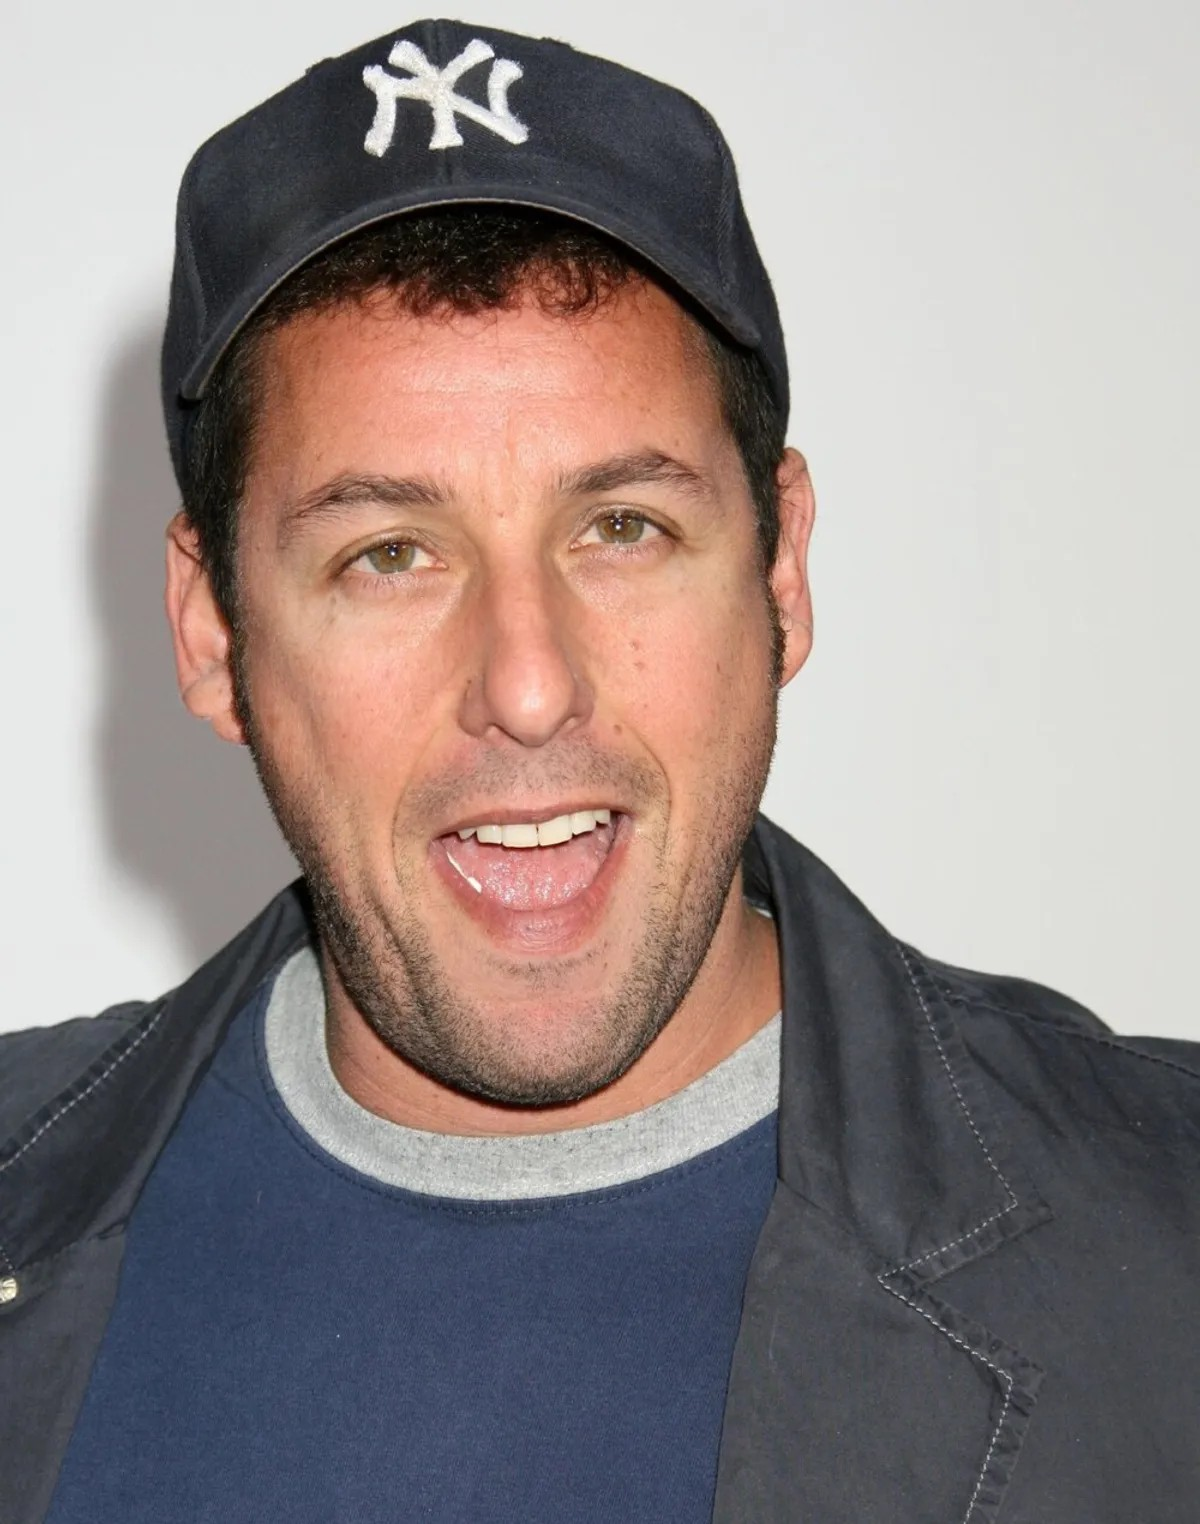
\includegraphics[width=\linewidth]{adam-sandler.jpg}};
        \end{scope}
        \draw[roxo,line width=0.9pt,rounded corners=2mm] (0,0) rectangle (\linewidth,1.27\linewidth);
        % Etiqueta inclinada por cima da foto
        \node[fill=roxo,text=white,font=\footnotesize\bfseries,rounded corners=1mm,
              inner xsep=2mm,inner ysep=1.2mm,rotate=-6,drop shadow={opacity=0.35}]
          at (0.5\linewidth,0.16\linewidth) {Não esse Adam};
      \end{tikzpicture}
    \end{column}
  \end{columns}
  \vspace{4mm}
  \conclusao{Nos testes do grupo, SGD puro não fez o CartPole aprender em tempo razoável; com Adam, ele aprende.}
\end{frame}

% ---------------------------------------------------------------------
% 12. Parte 5
{\lavanda
\begin{frame}{Experience replay: treinar com memórias embaralhadas}{PARTE 5 · DQN.Replay}
  \begin{grade}{2}
    \begin{cartao}\ct{O problema}{Passos seguidos diferem só por 0,02 s de física. Treinar com eles em sequência faz a rede decorar uma região e esquecer o resto.}\end{cartao}
    \begin{cartao}\ct{A solução}{Guardar cada transição $(s, a, r, s', \mathit{done})$ e sortear minibatches de 32, uniformes e com reposição.}\end{cartao}
    \begin{cartao}\ct{Memória FIFO de 10.000}{Quando enche, sai a transição mais antiga, gerada por uma política pior.}\end{cartao}
    \begin{cartao}\ct{\texttt{Data.Sequence}}{\texttt{Seq.index} é $O(\log n)$; com lista e \texttt{!!}, sortear de 10.000 itens seria lento.}\end{cartao}
  \end{grade}
\end{frame}
}

% ---------------------------------------------------------------------
% 13. Parte 6
\begin{frame}{$\varepsilon$-greedy: explorar no começo, aproveitar depois}{PARTE 6 · DQN.Policy}
  % Miniatura no canto superior direito
  \begin{tikzpicture}[remember picture,overlay]
    \foreach \img [count=\k from 0] in {eps-1.jpg} {
      \begin{scope}[shift={([xshift=-9mm,yshift=-5mm]current page.north east)}]
        \begin{scope}
          \clip[rounded corners=1mm] (-10mm,-10mm) rectangle (0,0);
          \node[anchor=north east,inner sep=0pt] at (0,0) {\includegraphics[width=10mm]{\img}};
        \end{scope}
        \draw[roxo,line width=0.6pt,rounded corners=1mm] (-10mm,-10mm) rectangle (0,0);
      \end{scope}
    }
  \end{tikzpicture}%
  \begin{columns}[c,onlytextwidth]
    \begin{column}{0.46\textwidth}
      \begin{tikzpicture}
        \begin{axis}[estilo, width=6.6cm, height=4.6cm,
            xmin=0, xmax=14000, scaled x ticks=false, ymin=0, ymax=1.08,
            xtick={10000}, xticklabels={10.000 passos},
            ytick={0.05,1}, yticklabels={0{,}05, 1{,}0},
            ylabel={$\varepsilon$}, ylabel style={rotate=-90},
            xlabel={passos $\to$}, xlabel style={at={(0.12,0)},anchor=north}]
          \addplot[cinza!60,dashed,domain=0:14000] {0.05};
          \addplot[roxo,line width=1.4pt] coordinates {(0,1) (10000,0.05) (14000,0.05)};
          \addplot[only marks,mark=*,mark size=2pt,laranja] coordinates {(10000,0.05)};
        \end{axis}
      \end{tikzpicture}
    \end{column}
    \begin{column}{0.50\textwidth}
      \begin{grade}{1}
        \begin{cartao}\ct{Sorteia $u$ em $[0, 1)$}{Se $u < \varepsilon$, ação aleatória; senão, a de maior Q.}\end{cartao}
        \begin{cartao}\ct{Decai por passo}{Linear de 1,0 a 0,05 em 10.000 passos, não por episódio.}\end{cartao}
        \begin{cartao}\ct{Nunca chega a zero}{5\% de exploração continua para sempre.}\end{cartao}
      \end{grade}
    \end{column}
  \end{columns}
\end{frame}

% ---------------------------------------------------------------------
% 14. Parte 7: duas redes
{\lavanda
\begin{frame}{Duas redes: uma aprende, a outra segura o alvo}{PARTE 7 · DQN.Agent}
  \begin{grade}{2}
    \begin{cartao}\rotulo{REDE ONLINE}\ct{Escolhe as ações e é treinada}{Atualizada pelo Adam a cada passo de treino.}\end{cartao}
    \begin{cartaoD}\rotulo{REDE TARGET}\ct{Cópia congelada que calcula o alvo}{Recebe uma cópia da online a cada 500 passos.}\end{cartaoD}
  \end{grade}
  \vspace{3mm}
  \begin{grade}{2}
    \begin{cartao}\ct{Por que a target existe}{Se o alvo viesse da própria online, ele mudaria a cada atualização: a rede perseguiria o próprio rabo.}\end{cartao}
    \begin{cartao}\ct{\texttt{agentBest} guarda a melhor rede}{O DQN pode piorar depois de aprender. Guardamos a rede com a melhor média dos últimos 20 episódios.}\end{cartao}
  \end{grade}
\end{frame}
}

% ---------------------------------------------------------------------
% 15. Parte 7: runEpisode
\begin{frame}{\texttt{runEpisode}: o que acontece a cada passo}{PARTE 7 · DQN.Agent}
  \begin{grade}{1}
    \etapa{1}{$\varepsilon = $ \texttt{epsilonAt}(passos totais); a ação sai de \texttt{epsilonGreedy} com a rede online.}
    \etapa{2}{\texttt{stepEnv} dá o próximo estado; a transição entra no replay buffer.}
    \etapa{3}{O contador de passos totais sobe 1.}
    \etapa{4}{Com 500 ou mais transições no buffer (warmup), sorteia 32 e roda \texttt{trainStep}.}
    \etapa{5}{Se os passos totais são múltiplo de 500, target := online.}
  \end{grade}
  \vspace{3mm}
  \conclusao{Haskell é preguiçoso: \texttt{force} (deepseq) e \texttt{BangPatterns} a cada passo evitam acumular milhões de cálculos pendentes.}
\end{frame}

% ---------------------------------------------------------------------
% 16. Hiperparâmetros
{\lavanda
\begin{frame}{Hiperparâmetros do treino}{CONFIGURAÇÃO · defaultHyperparams}
  \scriptsize\renewcommand{\arraystretch}{1.3}
  \begin{tabularx}{\textwidth}{@{}p{0.3\textwidth}p{0.2\textwidth}X@{}}
    \toprule
    \cab{Parâmetro} & \cab{Valor} & \cab{Para que serve}\\
    \midrule
    Camadas da rede        & \texttt{[4, 64, 2]}       & Entrada, oculta e saída\\
    $\gamma$ (desconto)    & 0,99                      & Peso dos pontos futuros\\
    Taxa de aprendizado    & 0,001                     & Tamanho do passo do Adam\\
    Minibatch              & 32                        & Transições por passo de treino\\
    Capacidade do buffer   & 10.000                    & Tamanho da memória\\
    Warmup                 & 500                       & Transições antes de treinar\\
    Sincronizar a target   & a cada 500 passos         & Estabiliza o alvo\\
    $\varepsilon$          & 1,0 $\to$ 0,05            & Em 10.000 passos, linear\\
    Máximo por episódio    & 500 passos                & Limite de uma partida\\
    Episódios              & 400                       & Duração do treino\\
    Janela da melhor rede  & 20 episódios              & Média móvel do \texttt{agentBest}\\
    \bottomrule
  \end{tabularx}
\end{frame}
}

% ---------------------------------------------------------------------
% 17. Resultados
{\escuro
\begin{frame}{Resultados: média de passos em 20 episódios}{PARTE 8 · DQN.Experiment}
  \begin{grade}{3}
    \begin{cartaoE}\rotulo{POLÍTICA ALEATÓRIA}\numero{21,35}{\color{cinzaclaro}A referência: agir ao acaso.}\end{cartaoE}
    \begin{cartaoE}\rotulo{REDE FINAL}\numero{196,40}{\color{cinzaclaro}A rede depois dos 400 episódios.}\end{cartaoE}
    \begin{cartaoED}\rotulo{MELHOR REDE · agentBest}\numero{192,75}{\color{cinzaclaro}Cerca de 9 vezes a aleatória.}\end{cartaoED}
  \end{grade}
  \vspace{1mm}
  \begin{tikzpicture}
    \begin{axis}[estilo, width=\linewidth, height=2.9cm,
        axis lines=left, axis line style={draw=none}, xmin=1, xmax=400, ymin=0, ymax=215,
        ytick={0,100,200}, xtick={1,100,200,300,400},
        xticklabels={1,100,200,300,episódio 400},
        ymajorgrids, grid style={marinho3},
        tick label style={font=\tiny\color{cinzaclaro}}, clip=false]
      \addplot[lilas,line width=1.1pt] table[x=episodio,y=media] {media-movel.dat};
      \node[font=\tiny,lilas,anchor=south] at (axis cs:327,184.35) {pico: 184,35};
    \end{axis}
  \end{tikzpicture}\par
  {\tiny\color{cinzaclaro}Semente 42, 400 episódios. Média móvel de 20 episódios do treino (com exploração): de cerca de 20 passos ao pico de 184,35. Avaliação dos cartões sem exploração.\par\vspace{0.6mm}
  Semente 1: rede final 12,65 e melhor rede 296,55. É a instabilidade do DQN, e por isso guardamos \texttt{agentBest}.}
\end{frame}
}

% ---------------------------------------------------------------------
% 18. Limitações e variantes
{\lavanda
\begin{frame}{O que o DQN não resolve, e como foi melhorado}{PARTE 9 · LIMITAÇÕES E VARIANTES}
  % Arco-íris no canto superior direito (o fundo branco da imagem foi removido)
  \begin{tikzpicture}[remember picture,overlay]
    \node[anchor=north east,inner sep=0pt] at ([xshift=-4mm,yshift=-3mm]current page.north east)
      {
\includegraphics[width=3.4cm]{arco-iris.png}};
  \end{tikzpicture}%
  \begin{columns}[t,onlytextwidth]
    \begin{column}{0.485\textwidth}
      {\ttfamily\tiny\bfseries\color{roxo}LIMITAÇÕES}\par\vspace{1.5mm}
      \begin{grade}{1}
        \begin{cartao}\ct{Instabilidade}{Pode piorar depois de aprender; por isso o \texttt{agentBest}.}\end{cartao}
        \begin{cartao}\ct{Superestimação}{O max no alvo tende a escolher erros para cima.}\end{cartao}
        \begin{cartao}\ct{Muitas amostras e ações discretas}{Precisa de muita interação e de um Q por ação.}\end{cartao}
      \end{grade}
    \end{column}
    \begin{column}{0.485\textwidth}
      {\ttfamily\tiny\bfseries\color{roxo}VARIANTES}\par\vspace{1.5mm}
      \begin{grade}{1}
        \begin{cartao}\ct{Double DQN}{Uma rede escolhe a ação, a outra avalia o valor.}\end{cartao}
        \begin{cartao}\ct{Dueling e Prioritized Replay}{Separa $V(s)$ e vantagem; sorteia mais as transições de maior erro TD.}\end{cartao}
        \begin{cartao}\ct{Rainbow}{Junta várias melhorias num só agente.}\end{cartao}
      \end{grade}
    \end{column}
  \end{columns}
\end{frame}
}

% ---------------------------------------------------------------------
% 19. Implementação
\begin{frame}{Por que Haskell puro, e o que isso exigiu}{IMPLEMENTAÇÃO}
  \begin{grade}{2}
    \begin{cartao}\ct{Nada é caixa-preta}{Sem bibliotecas de machine learning: só \texttt{base}, \texttt{containers}, \texttt{random} e \texttt{deepseq}. A rede é feita com listas.}\end{cartao}
    \begin{cartao}\ct{Código puro}{A aleatoriedade é passada como \texttt{StdGen} e devolvida junto do resultado. \texttt{IO} só existe no Main.}\end{cartao}
    \begin{cartao}\ct{Preguiça sob controle}{\texttt{force} e \texttt{BangPatterns} a cada passo, para a memória não estourar.}\end{cartao}
    \begin{cartao}\ct{Testes em cada módulo}{Testes com hspec, incluindo a verificação numérica do gradiente. A CI roda \texttt{cabal test} em todo PR.}\end{cartao}
  \end{grade}
\end{frame}

% ---------------------------------------------------------------------
% 20. Encerramento
{\escuro
\begin{frame}
  \vspace*{2mm}
  {\ttfamily\tiny\bfseries\color{lilas}OBRIGADO}\par\vspace{2mm}
  {\fontsize{30}{33}\selectfont\bfseries Perguntas?}\par\vspace{3mm}
  {\small\color{cinzaclaro}Código, testes e textos teóricos de cada parte estão no repositório do grupo.}\par
  \vspace{14mm}
  {\ttfamily\tiny\bfseries\color{lilas}REFERÊNCIAS}\par\vspace{1.2mm}
  {\tiny\color{cinzaclaro}
  Mnih, V. et al. (2015). Human-level control through deep reinforcement learning. \emph{Nature}, 518.\par
  Sutton, R. S.; Barto, A. G. (2018). \emph{Reinforcement Learning: An Introduction}. 2ª ed. MIT Press.\par
  Barto, A. G.; Sutton, R. S.; Anderson, C. W. (1983). Neuronlike adaptive elements… \emph{IEEE SMC}.\par
  Kingma, D. P.; Ba, J. (2014). Adam: A Method for Stochastic Optimization. \emph{arXiv}.\par
  Lin, L.-J. (1992). Self-improving reactive agents based on reinforcement learning. \emph{Machine Learning}.\par}
  \vspace*{4mm}
\end{frame}
}

\end{document}
